% !TeX spellcheck = en_US
\chapter{Goal-based RL}
All human and robot's actions follow a certain goal. Goal tracking is as old as target tracking in control engineering \cite{mcdermott1992robot}. However, in many cases, the robot is programmed to follow a hidden goal inside the mind of the engineers. In other words, the robots or agents do not aware of the existence of the goals. They do, however, receive cues, usually in the form of cost functions, whether the goals is close or not. A more proactive learning approach would be to explicitly let the robots know of the goals while learning.

Goal-conditioned learning provides a harder, but more general problem setting. Instead of communicating \textit{how} to perform a single task, we communicate only \textit{what} needs to be done by providing the goals, which can be the desired observations of world states (single data point or a sparse/dense sequence of data). Given the goal, the agent is required to infer how to perform the task by itself. In psychology, this is known as \textit{observational learning} \cite{bandura1977social}. The task might not be finished in an optimal way, but sometimes it's more important that the task is completed. In addition, it's easier for the expert to demonstrate multiple tasks quickly and easily. \cite{pathak2018zero}

Two helpful literature surveys:
\begin{itemize}
	\item \citeaustitle{liu2022goal}
	\item \citeaustitle{colas2022autotelic}
\end{itemize}

\section{Introduction}
A goal is similar to \textit{terminal-reward function} $ z: \mathcal{S} \rightarrow \mathbb{R} $, which is the reward received if termination occurs at state $s$ \cite{sutton2011horde}. Early work has proposed policy and value network conditioned on different goals. \cite{schaul2015universal}
\begin{align}
	&g \in \mathcal{G} && \text{space of possible goal}\ \mathcal{G}\\
	&m_g: \mathcal{S} \rightarrow \mathcal{G} && \text{mapping from state space to goal space}\\
	&u_{g}: \mathcal{S} \times \mathcal{A} \rightarrow \mathbb{R} && \text{goal-conditioned reward function}\\
	&\pi: \mathcal{S} \times \mathcal{G} \rightarrow \mathcal{A} && \text{goal-conditioned policy}\\
	&Q_{\pi}(s_t, a_t, g) = \mathbb{E}_{\pi}[r_t | s_t, a_t, g] && \text{goal-conditioned Q function}
\end{align}
Comparing to other conventional \ac{RL} approaches, goal-conditioned learning has various nice properties:
\begin{itemize}
	\item Off-policy learning
	\item Can be trained in a self-supervised / unsupervised manner for environment exploration
	\item Multi-task learning, \ac{aka} multi-goal learning
	\item Works well with sparse and binary reward.
	\item Has an implicit curriculum / can be extend to curriculum learning
\end{itemize}

\section{Reward Shaping}
Reward is basically the dopamine of \ac{RL}. It's the feedback from the environment that let the model know which are the desired behaviors to be enforced. Reward shaping is the step in which we design the reward function for our \ac{MDP}. Most of the time, it is complicate and requires domain knowledge. Inverse \ac{RL} is another direction to learn complex reward function from expert's demonstration. Goal-conditioned learning provides an elegant and easy way to tackle reward shaping. The example is the 
\ac{HER}, a goal-conditioned \ac{RL} framework for problems with sparse and binary reward \cite{andrychowicz2017hindsight}.

\begin{itemize}
	\item Normally, the transitions $ (\textbf{s}, \textbf{a} ,\textbf{s}', r)_i $ is added to the buffer
	\item \ac{HER} adds the transition with both desired and actually reached goals:
	\begin{itemize}
		\item $ (\textbf{s}, \textbf{a} ,\textbf{s}', g_{desired}, -1)_i $. Since the desired goal is not reached, the reward is $ r=-1 (\text{or } 0) $
		\item $ (\textbf{s}, \textbf{a} ,\textbf{s}', g_{actual}, 1)_i $. The transition with actual goal has positive binary reward $ r=1 $
	\end{itemize}
	\item Add some exploration, even more than count-based exploration
	\item Reward shaping may help, and it may not.
	\item \note Successful applications of \ac{RL} to difficult manipulation tasks which does not use
	demonstrations usually have more complicated reward functions (e.g. \cite{popov2017data}).
	\begin{itemize}
		\item There is a huge discrepancy between what we optimize and the success condition
		\item Shaped rewards penalize for inappropriate behavior which may hinder exploration.
	\end{itemize}
	\item Experiments compare performances of actor-critic (DDPG) \cite{lillicrap2015continuous} and Deep Q-networks (DQN) \cite{mnih2015human} with and without \ac{HER}
\end{itemize}

\section{Exploration}
The process of trying to reach different goals is equivalent with going to different states, which is exactly what exploration is about. Thus the more diverse and also gradually more challenging the goals are, the better the exploration scheme is. The goal can be sampled from:
\begin{itemize}
	\item the actual trajectories \cite{andrychowicz2017hindsight}.
	\item the complete distribution of the goals, which then it's required to learn that distribution. In \cite{nair2018visual}, \citeauthor*{nair2018visual} combine that with TD3 \cite{fujimoto2018addressing} (model-free Q-learning), with the reward as the negative Mahalanobis distance between the latent vectors of the goal and of the current state.
	\item Additional extension on the fact that the initial policy might stuck in local optima, which results in similar visited states. The goal/state distribution can be modified to prioritize less visited goals/states \cite{pong2019skew}
\end{itemize}
\begin{figure}[hbt!]
	\centering
	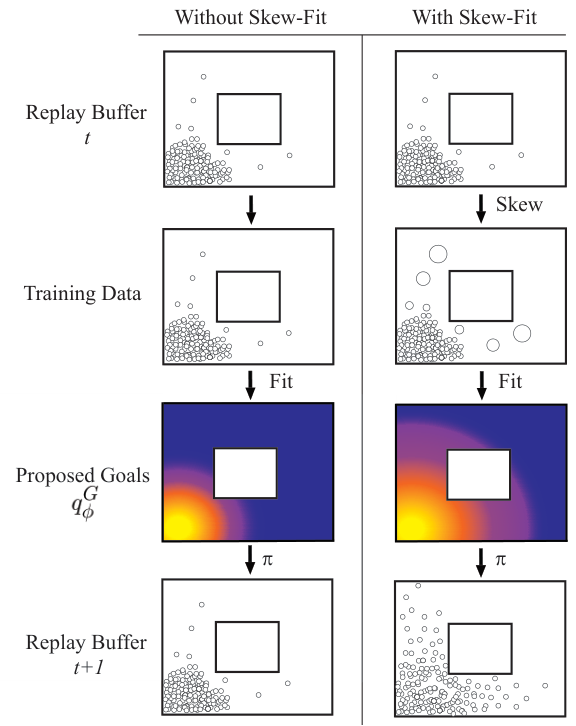
\includegraphics[width=.5\textwidth]{pong2020skewfit.png}
	\caption{Skewing the goal/state distribution to sample less visited ones. \cite{pong2019skew}}
\end{figure}

\section{Curriculum Learning}
Curriculum Learning is about how to gradually increase how challenging the goal is.
\begin{itemize}
	\item \ac{HER}'s extension: Curriculum-guided \ac{HER} \cite{fang2019curriculum}
\end{itemize}

\section{Sample Efficiency}
So far, compared to approaches not conditioned on the goals, most experiments of goal-conditioned learning also showed better sample efficiency when dealing with complex tasks. \cite{andrychowicz2017hindsight, nair2018visual}

\section{Learning Sequence of Subgoals}
Complex actions are sequence of more simple actions. \Eg:
\begin{itemize}
	\item Pouring a cup of water: grasp the bottle, move it above the cup, in-place rotate, put the bottle back.
	\item Make a cup of coffee: grasp the cup, move it to the coffee machine, put it in specified position, press the machine button \cite{smith2019avid}
\end{itemize}
One could certainly explicitly specify the subgoals / instructions for the robot to learn, either giving goal after goals, or pre-recording a (dense/sparse) sequence of subgoals \cite{pathak2018zero, smith2019avid}. However, there exists more elaborate schemes.

\subsection{Imagined Subgoals}
With the assumption that the goal space is the state space $ \mathcal{G} \equiv \mathcal{S} $, additional to an actor-critic model, a high-level policy $ \pi^{H}(.|s,g) $ predicts subgoals $ s_g $ \cite{chane2021goal}
\begin{itemize}
	\item Using value function $ V^{\pi}(s, g) $ to estimate the distance between valid states, define the subgoal $ s_g $ as midpoints on the path from $s$ to $g$. Minimize the cost:
	\begin{equation}
		C_{\pi}(s_g |s, g) = \max \left( V^{\pi}(s, s_g), V^{\pi}(s_g, g) \right)
	\end{equation}
	\item Enforce subgoal as valid state by \ac{KL}-divergence with actual valid state distribution $ p_s(.) $
	\begin{equation}
		D_{KL}\left( \pi^{H}(.|s, g) \;||\; p_s(.) \right) \leq \epsilon
	\end{equation}
	\item Policy of reaching final goal should be similar to reaching subgoals
	\begin{equation}
		D_{KL}\left( \pi(.|s, g) \;||\; \pi(.|s, s_g) \right) \leq \epsilon
	\end{equation}
\end{itemize}

\subsection{Learning from YouTube Videos}
Some proposals to model action plans using symbolic representation: $ Action(Object_1, Object_2, \dots) $
\begin{itemize}
	\item \citeaustitle{zhang2019robot}
	\item \citeaustitle{yang2015robot}
\end{itemize}
Action plans as symbolic representation  with visual sentence, \eg, $Grasp\_PoS(LeftHand,\ Spatula)$, $Action\_Stir(Spatula,\ Bowl)$

\section{Tips and Tricks}
\begin{itemize}
	\item Have a library of simple action primitives (in some problem settings, there is only 1 primitive). The model chooses an action from that library and/or output \ac{param} (as regression task) for that action primitive. \cite{pathak2018zero}\\
	Direct control leads to shaking artifacts in movements (\eg, \href{http://rll.berkeley.edu/dsae}{video1}, \href{https://sites.google.com/site/visualrlwithimaginedgoals}{video2}) \cite{nair2018visual}
	\item Whether how the task is finished is important
	\begin{itemize}
		\item If NOT: consider forward consistency loss \cite{pathak2018zero}
		\item If YES: ?
	\end{itemize}
	\item Model \& loss function:
	\begin{itemize}
		\item Binary reward \cite{andrychowicz2017hindsight}
		\item L2 loss in feature space? \cite{nair2018visual, pathak2018zero}
	\end{itemize}
\end{itemize}

\section{Experiments}
\subsection{RL Algorithms}
\begin{itemize}
	\item Imitation learning \cite{pathak2018zero}
	\item Actor-critic
	\begin{itemize}
		\item DDPG \cite{andrychowicz2017hindsight}
		\item \cite{chane2021goal}
	\end{itemize}
	\item Value-based RL
	\begin{itemize}
		\item DQN \cite{andrychowicz2017hindsight, nair2018visual}
	\end{itemize}
\end{itemize}

\subsection{Robotic Tasks}
\begin{itemize}
	\item Simple reaching task
	\item Object grasping/manipulation
	\begin{itemize}
		\item Object grasping \cite{andrychowicz2017hindsight, nair2018visual}
		\item Object pushing \cite{andrychowicz2017hindsight, nair2018visual, chane2021goal}
		\item Rope manipulation \cite{pathak2018zero}
		\item Door opening \cite{nair2018visual}
	\end{itemize}
	\item 2D/3D mobile robot navigation \cite{pathak2018zero, chane2021goal}
\end{itemize}

\section{References}
\begin{itemize}
	\item \citeaustitle{liu2022goal}
	\item \citeaustitle{pathak2018zero}
	\item \citeaustitle{andrychowicz2017hindsight}
	\item \citeaustitle{schaul2015universal}
\end{itemize}

Related other directions (maybe):
\begin{itemize}
	\item Brafman \etal \textit{"LTLf/LDLf Non-Markovian Rewards."}
	\item 	
\end{itemize}

\section{TODO}
\todo{check contextual policy}
\begin{itemize}
	\item M. P. Deisenroth, P. Englert, J. Peters, and D. Fox. Multi-task policy search for robotics. In International Conference on Robotics and Automation (ICRA), 2014.
	\item A. G. Kupcsik, M. P. Deisenroth, J. Peters, G. Neumann, et al. Data-efficient generalization of robot skills with contextual policy search. In AAAI Conference on Artificial Intelligence, 2013.
	\item F. Stulp, G. Raiola, A. Hoarau, S. Ivaldi, and O. Sigaud. Learning compact parameterized skills with a single regression. In International Confernce on Humanoid Robots, 2013.
	\item Y. Duan, M. Andrychowicz, B. Stadie, J. Ho, J. Schneider, I. Sutskever, P. Abbeel, and W. Zaremba. One-shot imitation learning. arXiv preprint arXiv:1703.07326, 2017.
\end{itemize}